%%% LaTeX Template: Article/Thesis/etc. with colored headings and special fonts
%%%
%%% Source: http://www.howtotex.com/
%%% Feel free to distribute this template, but please keep to referal to http://www.howtotex.com/ here.
%%% February 2011
%%%
%%% Last updated January 2018 by CDM

%%%  Preamble
\documentclass[11pt,letterpaper]{article}
\usepackage[margin=1.0in]{geometry}
\usepackage[T1]{fontenc}
\usepackage[bitstream-charter]{mathdesign}
\usepackage[latin1]{inputenc}					
\usepackage{amsmath}						
\usepackage{xcolor}
\usepackage{cite}
\usepackage{hyphenat}
\usepackage{graphicx}
\usepackage{float}
\usepackage{subfigure}
\usepackage{sectsty}
\usepackage[compact]{titlesec} 
\usepackage[tablegrid]{vhistory}
\usepackage{url}


\allsectionsfont{\color{accentcolor}\scshape\selectfont}

%%% Definitions
\definecolor{accentcolor}{rgb}{0.0,0.0,0.5} 
\newcommand{\teamname}{The Brew Crew}
\newcommand{\productname}{Beverage Management}
\newcommand{\coursename}{CSE 4316: Senior Design I}
\newcommand{\semester}{Summer 2020}
\newcommand{\docname}{Project Charter}
\newcommand{\department}{Department of Computer Science \& Engineering}
\newcommand{\university}{The University of Texas at Arlington}
\newcommand{\authors}{Bishal Paudel \\ Nirjal Phaiju \\ Sima Raymajhi \\ Lokendra B. Chhetri \\ Kunal Samant }

%%% Headers and footers
\usepackage{fancyhdr}
	\pagestyle{fancy}						% Enabling the custom headers/footers
\usepackage{lastpage}	
	% Header (empty)
	\lhead{}
	\chead{}
	\rhead{}
	% Footer
	\lfoot{\footnotesize \teamname \ - \semester}
	\cfoot{}
	\rfoot{\footnotesize page \thepage\ of \pageref{LastPage}}	% "Page 1 of 2"
	\renewcommand{\headrulewidth}{0.0pt}
	\renewcommand{\footrulewidth}{0.4pt}

%%% Change the abstract environment
\usepackage[runin]{abstract}			% runin option for a run-in title
%\setlength\absleftindent{30pt}			% left margin
%\setlength\absrightindent{30pt}		% right margin
\abslabeldelim{\quad}	
\setlength{\abstitleskip}{-10pt}
\renewcommand{\abstractname}{}
\renewcommand{\abstracttextfont}{\color{accentcolor} \small \slshape}	% slanted text

%%% Start of the document
\begin{document}

%%% Cover sheet
{\centering \huge \color{accentcolor} \sc \textbf{\department \\ \university} \par}
\vspace{1 in}
{\centering \huge \color{accentcolor} \sc \textbf{\docname \\ \coursename \\ \semester} \par}
\vspace{0.5 in}
\begin{figure}[h!]
	\centering
   	
\includegraphics[width=0.40\textwidth]{images/beverage}
\end{figure}
\vspace{0.5 in}
{\centering \huge \color{accentcolor} \sc \textbf{\teamname \\ \productname} \par}
\vspace{0.5 in}
{\centering \large \sc \textbf{\authors} \par}
\newpage


%\vspace{1 in}
%\centerline{January 13th, 2012}
%\newpage

%%% Revision History
\begin{versionhistory}
	  \vhEntry{0.1}{07.30.2020}{BP}{document creation}
	  \vhEntry{0.2}{07.30.2020}{BP}{section 1 added}
	  \vhEntry{0.4}{08.03.2020}{LC}{sections 4 and 5 added}
	  \vhEntry{0.3}{08.04.2020}{KS}{Section 2 added}
	  \vhEntry{0.3}{08.04.2020}{NP}{Section 3 added}
	  \vhEntry{0.3}{08.05.2020}{LC}{Section 6,7,8,9 added}
	  \vhEntry{0.4}{08.06.2020}{KS}{Section 2 diagrams added}
	  
\end{versionhistory}
\newpage

%%% Table of contents
\setcounter{tocdepth}{2}
\tableofcontents
\newpage

%%% List of figures and tables (optional)
\listoffigures
%\listoftables
\newpage

\section{Product Concept}
This section describes the purpose, use and intended user audience for the Beverage Management app. Beverage Management app is an android application that provides an efficient way to manage large collection of beverages using smartphone.

\subsection{Purpose and Use}
Beverage Management is an android application that works as a virtual inventory and allows user to effectively manage and keep track of several beverages. Users can use this app to keep track of name, storage location, brewery, style, volume, manufactured date and best before date. It also allows user to search and sort the beverages according to the date, style etc.

\subsection{Intended Audience}
The intended audience for this application are those people who have large collection of beverages in their home and are looking for easy ways to manage them free of cost. It can also be used in local grocery stores, bars and restaurants to keep track of their beverage inventory. Our app is intended for general use but it can certainly be expanded into a more complex inventory management system with additional features.  

\begin{figure}[h!]
	\centering
   	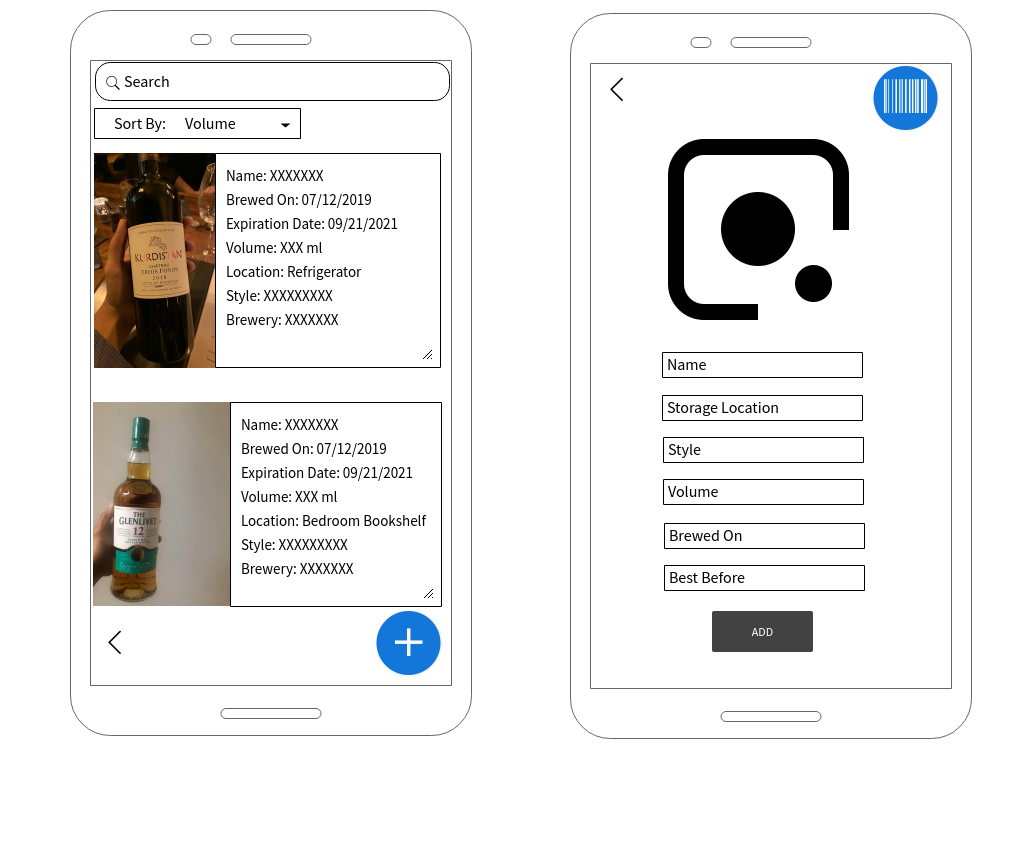
\includegraphics[width=0.60\textwidth]{images/CD.png}
    \caption{ conceptual drawing of Beverage Management App (Home screen and Add screen) }
\end{figure}

\newpage
\section{Product Description}
This section provides the reader with an overview of Beverage Management. Beverage Management is an Android 
application that manages the beverages which a user has stored in their storage space. the application will have access
to a dataset of various drinks (beers in the initial release) and have will be able to populate the virtual storage 
space as to simulate the actual storage of the user's drinks. The application will have a login functionality to allow 
users to personalize their experience. The application will also send notifications to alert the user of 
soon-to-expire drinks.

\subsection{Features \& Functions}
This product will help users manage and optimize their storage space and reduce wastage. The app will connect to a database,
primarily we will use firebase, which will store user information and beverage information. The beverage data will be extracted
using the barcode which the app can scan using the phone's camera.

\begin{figure}[h!]
	\centering
   	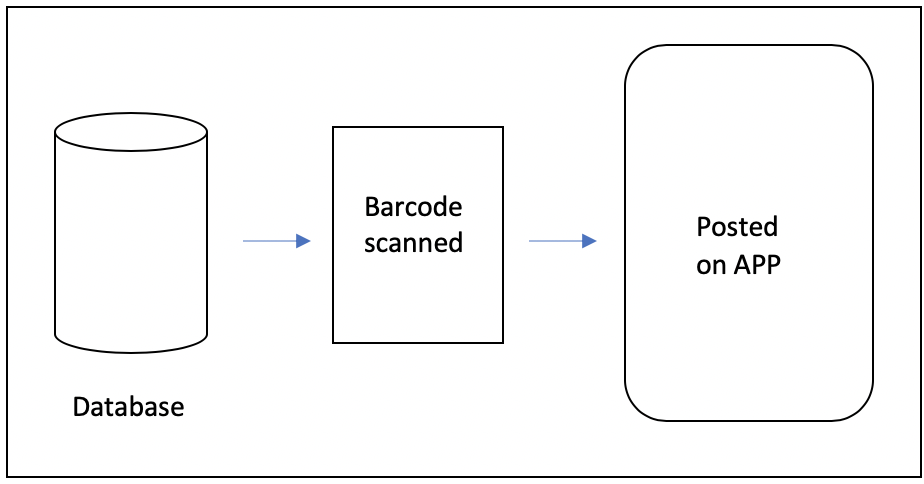
\includegraphics[width=0.60\textwidth]{images/bevearge_data_request.png}
    \caption{ Database Design }
\end{figure}

\subsection{External Inputs \& Outputs}
The users will scan the barcode of the drink, which will then access the dataset and output the details of the drink within the required storage area on the app.
Our app will extract the information as well, such as expiry date, and use it to send push notifications to the user.

\subsection{Product Interfaces}
We will have a default home screen which will display be modeled to copy Dr. Conly's storage area, in the initial release. There 
will be a button to access the camera and a settings page and an editing page as well.

\begin{figure}[h!]
	\centering
   	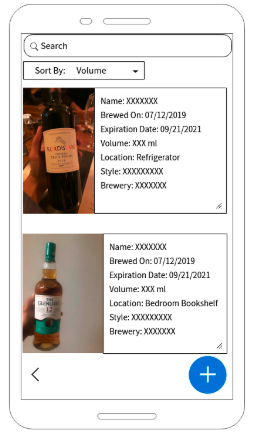
\includegraphics[width=0.60\textwidth]{images/home_screen.png}
    \caption{ Home Page after login (varies per user) }
\end{figure}
\newpage
\section{Customer Requirements}
Here, we have requirements that our group came up with after having a detailed conversation with our customer and group members. These requirements are documentation of what our customer expects from our mobile application and these requirements will not be changed without the consent of the customer. 

\subsection{Accurate Inventory Tracking}
\subsubsection{Description}
Customers shall be able to track the total number of a specific beer available in their inventory.
\subsubsection{Source}
Nirjal
\subsubsection{Constraints}
N/A
\subsubsection{Standards}
N/A
\subsubsection{Priority}
High

\subsection{An Attractive and easy to use User Interface}
\subsubsection{Description}
Customers shall be able to navigate through our application without any confusion and complications.
\subsubsection{Source}
Kunal
\subsubsection{Constraints}
N/A
\subsubsection{Standards}
N/A
\subsubsection{Priority}
High

\subsection{Successful access to the Camera}
\subsubsection{Description}
The application shall have no problem using the user's cellphone camera after getting user's consent.
\subsubsection{Source}
Kunal
\subsubsection{Constraints}
The user will have to put in the extra work in order to enter the product name and categorize it manually if the camera is not functioning properly.
\subsubsection{Standards}
N/A
\subsubsection{Priority}
Critical

\subsection{Login Functionality}
\subsubsection{Description}
The user shall be able to login to their account without any complications with correct username and password. In case user forgets the password, there shall be a way for the user to recover it.
\subsubsection{Source}
Lokendra
\subsubsection{Constraints}
N/A
\subsubsection{Standards}
N/A
\subsubsection{Priority}
Critical

\subsection{Search by Product Name, Brewery, and Beer style}
\subsubsection{Description}
The application shall be able to search and display the product that already exists in the inventory on the basis of product name, brewery, and beer style.
\subsubsection{Source}
Sima and Chris
\subsubsection{Constraints}
N/A
\subsubsection{Standards}
N/A
\subsubsection{Priority}
Critical

\subsection{Notification if the beer is nearing expiry date}
\subsubsection{Description}
The application shall notify the user about the products in the inventory that are nearing their best by date.
\subsubsection{Source}
Chris
\subsubsection{Constraints}
N/A
\subsubsection{Standards}
N/A
\subsubsection{Priority}
Critical

\subsection{Sort by best by date, brew date, and format}
\subsubsection{Description}
The application shall be able to sort the displayed items based on nearest expiration date, brew date and item size (12 oz. bottle, 12 oz. can, .33 L bottle, etc.).
\subsubsection{Source}
Chris
\subsubsection{Constraints}
N/A
\subsubsection{Standards}
N/A
\subsubsection{Priority}
High

\subsection{Create a Storage Location with NxM rows and columns}
\subsubsection{Description}
The application shall be able to create and save a storage location in the format of NxM rows and columns 
\subsubsection{Source}
Chris
\subsubsection{Constraints}
N/A
\subsubsection{Standards}
N/A
\subsubsection{Priority}
High

\subsection{Ability to take a picture of bottle/can to store that}
\subsubsection{Description}
The application shall allow user to click and save a photo of the item that we are storing.
\subsubsection{Source}
Chris
\subsubsection{Constraints}
N/A
\subsubsection{Standards}
N/A
\subsubsection{Priority}
Moderate

\subsection{Notes section to add any comments that user may find useful(example: Tasting Notes)}
\subsubsection{Description}
The application shall allow user to click and save a photo of the item that we are storing.
\subsubsection{Source}
Chris
\subsubsection{Constraints}
N/A
\subsubsection{Standards}
N/A
\subsubsection{Priority}
Low

\subsection{Warning when mobile storage space is low}
\subsubsection{Description}
The application shall warn users when mobile storage space is running low and the app cannot save anymore photos, notes, etc.
\subsubsection{Source}
Bishal
\subsubsection{Constraints}
N/A
\subsubsection{Standards}
N/A
\subsubsection{Priority}
Low
\newpage
\section{Packaging Requirements}
The application software shall be loaded to our client's mobile device. The client's preferred platform shall be android OS. Client/User can also download via google play store for free. Additionally, the application software shall be stored on team lead's external hard drive and GitHub repository.  

\subsection{Installing Application}
\subsubsection{Description}
The application will be installed in the client's device by private downloadable link provided by the team, the initial setup or installation must be required by the user.   
\subsubsection{Source}
Team
\subsubsection{Constraints}
User must have access to internet connectivity. 
\subsubsection{Standards}
N/A
\subsubsection{Priority}
High
\newpage
\section{Performance Requirements}
The application should be able to precisely scan the bar code and establish the connection with the saved beverages or add new beverage to the database. Adding a new self with required number of rows and columns for initial setup for the beverages should not take more than 1-2 minutes. 

\subsection{Accurate Barcode Scanning}
\subsubsection{Description}
The system should accurately scan the bar code with minimal number of errors.
\subsubsection{Source}
Team member
\subsubsection{Constraints}
Internet connectivity is important to make the connection with the database to match the scanned bar code. 
\subsubsection{Standards}
All information should be stored in the database. 
\subsubsection{Priority}
High


\newpage
\section{Safety Requirements}
The Development of Brew Crew project does not include any of the toxic chemicals, sharp objects or any laser beams so there  are no specific safety requirements for this project.The basic laboratory safety measures is listed below:

\subsection{Laboratory Equipment Lockout/Tagout (LOTO) Procedures}
\subsubsection{Description}
Any fabrication equipment provided used in the development of the project shall be used in accordance with OSHA standard LOTO procedures. Locks and tags are installed on all equipment items that present use hazards, and ONLY the course instructor or designated teaching assistants may remove a lock. All
locks will be immediately replaced once the equipment is no longer in use.
\subsubsection{Source}
CSE Senior Design laboratory policy
\subsubsection{Constraints}
Equipment usage, due to lock removal policies, will be limited to availability of the course instructor and designed teaching assistants.

\subsubsection{Standards}
 Occupational Safety and Health Standards 1910.147 - The control of hazardous energy (lockout/tagout).
\subsubsection{Priority}
Critical

\subsection{National Electric Code(NEC) Wiring Compliance}
\subsubsection{Description}
Any electrical wiring must be completed in compliance with all requirements specified in the National Electric Code. This includes wire runs, insulation, grounding, enclosures, over-current protection, and all other specifications.
\subsubsection{Source}
CSE Senior Design laboratory policy
\subsubsection{Constraints}
High voltage power sources, as defined in NFPA 70, will be avoided as much as possible in order to minimize potential hazards.
\subsubsection{Standards}
 NFPA 70

\subsubsection{Priority}
Critical

\subsection{RIA Robotic Manipulator Safety Standards}
\subsubsection{Description}
Robotic manipulators, if used, will either housed in a compliant lockout cell with all required safety interlocks, or certified as a "collaborative" unit from the manufacturer.

\subsubsection{Source}
CSE Senior Design laboratory policy
\subsubsection{Constraints}
Collaborative robotic manipulators will be preferred over non-collaborative units in order to minimize potential hazards. Sourcing and use of any required safety interlock mechanisms will be the responsibility of the engineering team.
\subsubsection{Standards}
 ANSI/RIA R15.06-2012 American National Standard for Industrial Robots and Robot
 Systems, RIA TR15.606-2016 Collaborative Robots
 
\subsubsection{Priority}
Critical


 

\newpage
\section{Maintenance \& Support Requirements}
Include a header paragraph specific to your product here. Maintenance and support requirements address items specific to the ongoing maintenance and support of your product after delivery. Think of these requirements as if you were the ones who would be responsible for caring for customers/end user after the product is delivered in its final form and in use "in the field". What would you require to do this job? Specify items such as: where, how and who must be able to maintain the product to correct errors, hardware failures, etc.; required support/troubleshooting manuals/guides; availability/documentation of source code; related technical documentation that must be available for maintainers; specific/unique tools required for maintenance; specific software/environment required for maintenance; etc.

\subsection{Requirement Name}
\subsubsection{Description}
Detailed requirement description...
\subsubsection{Source}
Source
\subsubsection{Constraints}
Detailed description of applicable constraints...
\subsubsection{Standards}
List of applicable standards
\subsubsection{Priority}
Priority
\newpage
\section{Other Requirements}

\subsection{The Source Code will be Portable }
\subsubsection{Description}
The Source code will be compatible on Windows, Linux and MAC System.
\subsubsection{Source}
Team
\subsubsection{Constraints}
N/A
\subsubsection{Standards}
N/A
\subsubsection{Priority}
Critical
\newpage
\section{Future Items}
In this last section, you will reiterate all requirements that are listed as priority 5. This is repetitive, but necessary as a concise statement of features/functions that were considered/discussed and documented herein, but will NOT be addressed in the prototype version of the product due to constraints of budget, time, skills, technology, feasibility analysis, etc. Use the following format for this section.

\subsection{Requirement Name}
\subsubsection{Description}
Detailed requirement description...
\subsubsection{Source}
Source
\subsubsection{Constraints}
Detailed description of applicable constraints...
\subsubsection{Standards}
List of applicable standards
\subsubsection{Priority}
Priority
\newpage

%%% References
\bibliographystyle{plain}
\bibliographystyle{reference/IEEEtran_custom}
\bibliography{reference/refs}{}

\end{document}